\chapter{Analysis}
\label{chap:analysis}

\lipsum[1]

\minitoc

\newpage

% -----------------------------------------------------------------------------
This chapter shows example of picture and also serves to populate the different lists: list of figures, list of tables, bibliography, and glossary.

\section{Tables}

This section contains an examples of table: \autoref{tab:esempio} and 

\begin{table}[H]
    \centering
    \begin{tabular}{ccc}
	\toprule
	name & weight & food \\ 
	\midrule
	mouse	& 10 g	& cheese \\
	cat	& 1 kg	& mice \\
	dog	& 10 kg	& cats \\
	\bottomrule 
    \end{tabular}
    \caption[A floating table]{A floating table.}
    \label{tab:esempio}
\end{table}

\section{Milestones}
\label{sec:milestones}

The project consists of several milestones along the way to lay the foundation for its progress.

\begin{table}[H]
    \centering
    \rowcolors{1}{Lavender!80!gray}{white}
    \begin{tabular}{|L{2.5cm}|L{2.5cm}|C{3cm}|}
        \hline
	\rowcolor{lightgray} \textbf{\large{Name}} & \textbf{\large{Weight}} & \textbf{\large{Food}} \\
	\hline
	mouse & 10g & cheese \\
	\hline
        cat & 1kg & mice \\
	\hline
        dog & 10kg & cats \\
	\hline
    \end{tabular}
    \caption{A pretty table}
\end{table}

\subsection{Figures}

This section contains examples of figures: \autoref{fig:galleria}, \autoref{fig:lorem}, \autoref{fig:ipsum}, \autoref{fig:dolor}, \autoref{fig:sit}

\begin{figure}[H] 
    \centering 
    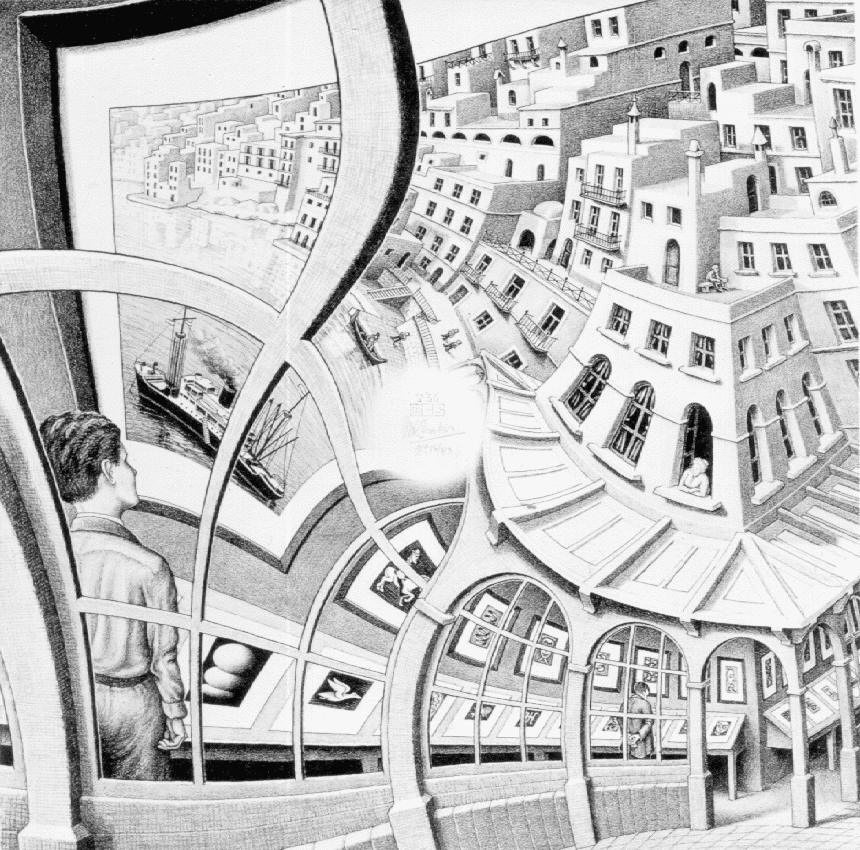
\includegraphics[width=0.3\columnwidth]{galleria_stampe.jpg} 
    \captionsource{A floating figure}{A floating figure: the lithograph \emph{Galleria di stampe}, of M.~Escher}{\url{http://www.mcescher.com/}}
    \label{fig:galleria} 
\end{figure}

\begin{figure}[H]
    \centering
    \begin{subfigure}[b]{0.45\textwidth}
	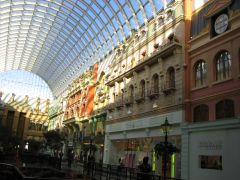
\includegraphics[width=\textwidth]{lorem.jpg}
	\caption{A gull}
        \label{fig:lorem}
    \end{subfigure}
    ~ %add desired spacing between images, e. g. ~, \quad, \qquad, \hfill etc. 
    %(or a blank line to force the subfigure onto a new line)
    \begin{subfigure}[b]{0.45\textwidth}
	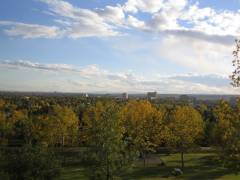
\includegraphics[width=\textwidth]{ipsum.jpg}
	\caption{A tiger}
	\label{fig:ipsum}
    \end{subfigure}
    ~ %add desired spacing between images, e. g. ~, \quad, \qquad, \hfill etc. 
    %(or a blank line to force the subfigure onto a new line)
    \begin{subfigure}[b]{0.45\textwidth}
	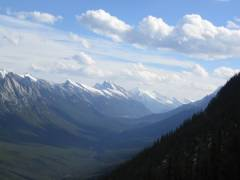
\includegraphics[width=\textwidth]{dolor.jpg}
	\caption{A mouse}
	\label{fig:dolor}
    \end{subfigure}
    ~ %add desired spacing between images, e. g. ~, \quad, \qquad, \hfill etc. 
    %(or a blank line to force the subfigure onto a new line)
    \begin{subfigure}[b]{0.45\textwidth}
	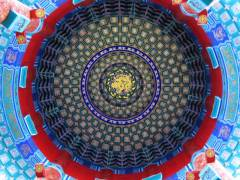
\includegraphics[width=\textwidth]{sit.jpg}
	\caption{A mouse}
	\label{fig:sit}
    \end{subfigure}
    \caption{Example subcaption}\label{fig:animals}
\end{figure}


% -----------------------------------------------------------------------------
\subsection{Code}

\autoref{lst:listing_example} shows an example of Java code rendered with minted.

\begin{listing}[H]
    \javafile{structure/listings/HelloWorld.java}
    \caption{Example of listing using the minted package}
    \label{lst:listing_example}
\end{listing}

% -----------------------------------------------------------------------------
\subsection{Boxes}

There is the possibility to insert custom boxes like information or warning wise.

\begin{info}
    This is an important information.
\end{info}

\begin{warning}
    Attention! This is a warning!
\end{warning}

% -----------------------------------------------------------------------------
\subsection{Other features}

Term (glossaries): \gls{nosql}

Acronym (glossaries): \gls{sql}

Citation (biblatex): \cite{paper_millwheel}

% -----------------------------------------------------------------------------
\section{Conclusion}

\blindtext
